\begin{figure}
\centering
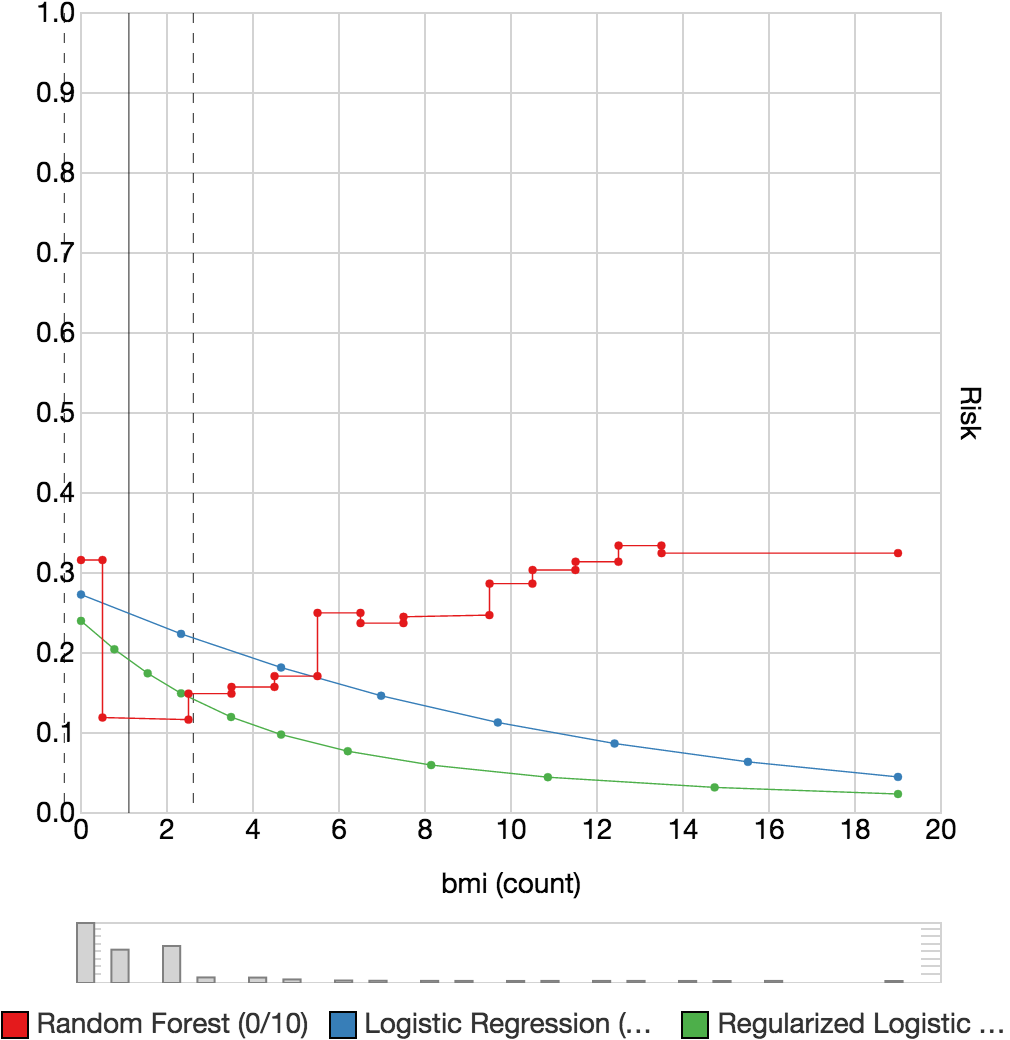
\includegraphics[width=0.7\linewidth]{prospector/cmp_bmi} % 0.8
\caption[Comparison of three machine learning models on the number of measured BMI values.]{
Comparison of three machine learning models on the number of measured BMI values.
The two regression models (logistic regression in blue and regularized logistic regression in green)
can express only a single slope (downwards or upwards) whereas the random forest in red can
model the strong decrease in predicted risk going from no BMI measures to one measure as well as
the later increase again if a patient has several BMI measures.
The random forest is more expressive, but the distribution of input values in the histogram below the plot hint the model might be overfitting as most of the observed values are 2 or less.
}
\label{figs:cmp_bmi}
\end{figure}